\documentclass{../mathhomework}
\usepackage{enumitem}
\usepackage{graphicx}
\usepackage{float}

\newcommand{\Let}{\textit{let }}
\newcommand{\Span}[1]{\textit{Span}\{#1\}}
\newcommand{\Powerset}[1]{\mathcal{P}(#1)}
\newcommand{\By}[1]{\text{(by #1)}}
\newcommand{\circnum}[1]{\text{\textcircled{#1}}}

\newenvironment{Mat}{\begin{bmatrix}}{\end{bmatrix}}

% Assigment Info
\coursetitle{Linear Algebra}
\courseinstructor{Professor MacArthur}

\student{Carson Storm}

\assignmenttitle{Homework \#2}
\assignmentduedate{September 4, 2019}

% Section 1.6 #4, 7, 11, 13
% Section 1.7 #1, 3, 5, 7, 11, 13, 15, 17, 19, 21, 23, 25
% Section 1.8 #1, 2, 3, 5, 7, 9, 11, 13, 16, 30, 33

\begin{document}
\maketitle

\pagebreak

\begin{problem}[1.6\#4]
    Suppose an economy has four sectors, Agriculture (A), Energy (E), Manufacturing (M), and Transportation (T). 
    Sector A sells 10\% of its output to E and 25\% to M and reatins the rese. Sectore E sells 30\% of its output
    to A, 35\% to M, and 25\% to T and reatins the rest. Sector M sells 30\% of its output to A, 15\% to E, and 40\%
    to T and reatins the rest. Sector T sells 20\% of its output to A, 10\% to E, and 30\% to M and retains the rest.
    \begin{enumerate}[label=\alph*.]
        \item Construct the exchange table for this economy.
        \item $[M]$ Find a set of equilibrium prices for the economy.
    \end{enumerate}

    \begin{solution}[Part A:]
        \begin{table}[h!]
            \begin{tabular}{|c|c|c|c|c|}
            \hline
            A    & E    & M    & T    & Purchased By \\ \hline
            0.65 & 0.30 & 0.30 & 0.20 & A            \\ \hline
            0.10 & 0.10 & 0.15 & 0.10 & E            \\ \hline
            0.25 & 0.35 & 0.15 & 0.30 & M            \\ \hline
            0.00 & 0.25 & 0.40 & 0.40 & T            \\ \hline
            \end{tabular}
        \end{table}
    \end{solution}

    \begin{solution}[Part B:]
        \begin{align*}
            \begin{Bmatrix}
                p_a = 0.65p_a + 0.30p_e + 0.30p_m + 0.20p_t \\
                p_e = 0.10p_a + 0.10p_e + 0.15p_m + 0.10p_t \\
                p_m = 0.25p_a + 0.35p_e + 0.15p_m + 0.30p_t \\
                p_t = 0.00p_a + 0.25p_e + 0.40p_m + 0.40p_t
            \end{Bmatrix} & \equiv
            \begin{Bmatrix}
                0 = -0.35p_a + 0.30p_e + 0.30p_m + 0.20p_t \\
                0 = 0.10p_a - 0.90p_e + 0.15p_m + 0.10p_t \\
                0 = 0.25p_a + 0.35p_e - 0.85p_m + 0.30p_t \\
                0 = 0.00p_a + 0.25p_e + 0.40p_m - 0.60p_t
            \end{Bmatrix} \\ & \equiv
            \begin{Mat}
                -0.35 & 0.30 & 0.30 & 0.20 & 0 \\
                0.10 & -0.90 & 0.15 & 0.10 & 0 \\
                0.25 & 0.35 & -0.85 & 0.30 & 0 \\
                0.00 & 0.25 & 0.40 & -0.60 & 0
            \end{Mat} \\ & \equiv
            \begin{Mat}
                1 & 0 & 0 & -2.0279 & 0 \\
                0 & 1 & 0 & -0.5311 & 0 \\
                0 & 0 & 1 & -1.1681 & 0 \\
                0 & 0 & 0 & 0 & 0 \\
            \end{Mat} \\ & \equiv
            \begin{Bmatrix}
                p_a = 2.0279p_t \\
                p_e = 0.5311p_t \\
                p_m = 1.1681p_t \\
                p_t = p_t
            \end{Bmatrix}
        \end{align*}

        The set of all equilibrium prices are
        \begin{equation*}
            \Vect{p} = p_t \begin{Mat}
                2.0279 \\ 0.5311 \\ 1.1681 \\ 1
            \end{Mat}
        \end{equation*}
    \end{solution}
\end{problem}

\begin{problem}[1.6\#7]
    Alka-Seltzer contains sodium bicarbonate ($NaHCO_3$) and citric acid ($H_3C_6H_5O_7$). When a tablet is dissolved
    in water, the following reaction produces sodium citrate, water, and carbon dioxide (gas):
    \begin{equation*}
        NaHCO_3 + H_3C_6H_5O_7 \to Na_3C_6H_5O_7 + H_2O + CO_2
    \end{equation*}
    Balance the chemical equaion using the vector equation approach.

    \begin{solution}
        \begin{equation*}
            NaHCO_3: \begin{Mat}
                1 \\ 1 \\ 1 \\ 3
            \end{Mat},
            H_3C_6H_5O_7: \begin{Mat}
                0 \\ 8 \\ 6 \\ 7
            \end{Mat},
            Na_3C_6H_5O_7: \begin{Mat}
                3 \\ 5 \\ 6 \\ 7
            \end{Mat},
            H_2O: \begin{Mat}
                0 \\ 2 \\ 0 \\ 1
            \end{Mat},
            CO_2: \begin{Mat}
                0 \\ 0 \\ 1 \\ 2
            \end{Mat}
        \end{equation*}
    \end{solution}

    So the vector equation that represents the reaction is
    \begin{equation*}
        x_1 \begin{Mat}
            1 \\ 1 \\ 1 \\ 3
        \end{Mat} + x_2 \begin{Mat}
            0 \\ 8 \\ 6 \\ 7
        \end{Mat} = x_3 \begin{Mat}
            3 \\ 5 \\ 6 \\ 7
        \end{Mat} + x_4 \begin{Mat}
            0 \\ 2 \\ 0 \\ 1
        \end{Mat} + x_5 \begin{Mat}
            0 \\ 0 \\ 1 \\ 2
        \end{Mat}
    \end{equation*}

    This is equivalent to the augmented matrices
    \begin{align*}
        \begin{Mat}
            1 & 0 & -3 & 0 & 0 & 0 \\
            1 & 8 & -5 & -2 & 0 & 0 \\
            1 & 6 & -6 & 0 & -1 & 0 \\
            3 & 7 & -7 & -1 & -2 & 0
        \end{Mat} & \equiv
        \begin{Mat}
            1 & 0 & -3 & 0 & 0 & 0 \\
            0 & 8 & -2 & -2 & 0 & 0 \\
            1 & 6 & -6 & 0 & -1 & 0 \\
            3 & 7 & -7 & -1 & -2 & 0
        \end{Mat} 
        \\ & \qquad{} R_2 = R_2 - R_1 \\
        \equiv \begin{Mat}
            1 & 0 & -3 & 0 & 0 & 0 \\
            0 & 8 & -2 & -2 & 0 & 0 \\
            0 & 6 & -3 & 0 & -1 & 0 \\
            3 & 7 & -7 & -1 & -2 & 0
        \end{Mat} 
        & \equiv \begin{Mat}
            1 & 0 & -3 & 0 & 0 & 0 \\
            0 & 8 & -2 & -2 & 0 & 0 \\
            0 & 6 & -3 & 0 & -1 & 0 \\
            0 & 7 & 2 & -1 & -2 & 0
        \end{Mat} \\
        R_3 = R_3 - R_1 & \qquad{} R_4 = R_4 - 4R_1 \\
        \equiv \begin{Mat}
            1 & 0 & -3 & 0 & 0 & 0 \\
            0 & 1 & -\frac{1}{4} & -\frac{1}{4} & 0 & 0 \\
            0 & 6 & -3 & 0 & -1 & 0 \\
            0 & 7 & 2 & -1 & -2 & 0
        \end{Mat}
        & \equiv \begin{Mat}
            1 & 0 & -3 & 0 & 0 & 0 \\
            0 & 1 & -\frac{1}{4} & -\frac{1}{4} & 0 & 0 \\
            0 & 6 & -3 & 0 & -1 & 0 \\
            0 & 0 & \frac{15}{4} & \frac{3}{4} & -2 & 0
        \end{Mat} \\
        R_2 = R_2/8 & \qquad{} R_4 = R_4 - 7R_2 \\
        \equiv \begin{Mat}
            1 & 0 & -3 & 0 & 0 & 0 \\
            0 & 1 & -\frac{1}{4} & -\frac{1}{4} & 0 & 0 \\
            0 & 0 & -\frac{3}{2} & \frac{3}{2} & -1 & 0 \\
            0 & 0 & \frac{15}{4} & \frac{3}{4} & -2 & 0
        \end{Mat}
        & \equiv \begin{Mat}
            1 & 0 & -3 & 0 & 0 & 0 \\
            0 & 1 & -\frac{1}{4} & -\frac{1}{4} & 0 & 0 \\
            0 & 0 & 1 & -1 & \frac{2}{3} & 0 \\
            0 & 0 & \frac{15}{4} & \frac{3}{4} & -2 & 0
        \end{Mat}  \\
        R_3 = R_3 - 6R_2 & \qquad{} R_3 = -2R_3/3 \\
        \equiv \begin{Mat}
            1 & 0 & -3 & 0 & 0 & 0 \\
            0 & 1 & -\frac{1}{4} & -\frac{1}{4} & 0 & 0 \\
            0 & 0 & 1 & -1 & \frac{2}{3} & 0 \\
            0 & 0 & 0 & \frac{9}{2} & -\frac{9}{2} & 0
        \end{Mat}
        & \equiv \begin{Mat}
            1 & 0 & -3 & 0 & 0 & 0 \\
            0 & 1 & -\frac{1}{4} & -\frac{1}{4} & 0 & 0 \\
            0 & 0 & 1 & -1 & \frac{2}{3} & 0 \\
            0 & 0 & 0 & 1 & -1 & 0
        \end{Mat} \\
        R_4 = R_4 -\frac{15}{4}R_3 & \qquad{} R_4 = 2R_4/9 \\
        \equiv \begin{Mat}
            1 & 0 & -3 & 0 & 0 & 0 \\
            0 & 1 & -\frac{1}{4} & -\frac{1}{4} & 0 & 0 \\
            0 & 0 & 1 & 0 & -\frac{1}{3} & 0 \\
            0 & 0 & 0 & 1 & -1 & 0
        \end{Mat}
        & \equiv \begin{Mat}
            1 & 0 & -3 & 0 & 0 & 0 \\
            0 & 1 & -\frac{1}{4} & 0 & -\frac{1}{4} & 0 \\
            0 & 0 & 1 & 0 & -\frac{1}{3} & 0 \\
            0 & 0 & 0 & 1 & -1 & 0
        \end{Mat} \\
        R_3 = R_3 + R_4 & \qquad{} R_2 = R_2 + R_4/4 \\
        \equiv \begin{Mat}
            1 & 0 & -3 & 0 & 0 & 0 \\
            0 & 1 & 0 & 0 & -\frac{1}{6} & 0 \\
            0 & 0 & 1 & 0 & -\frac{1}{3} & 0 \\
            0 & 0 & 0 & 1 & -1 & 0
        \end{Mat}
        & \equiv \begin{Mat}
            1 & 0 & 0 & 0 & -1 & 0 \\
            0 & 1 & 0 & 0 & -\frac{1}{3} & 0 \\
            0 & 0 & 1 & 0 & -\frac{1}{3} & 0 \\
            0 & 0 & 0 & 1 & -1 & 0 \\
        \end{Mat} \\
        R_2 = R_2 - R_3/4 & \qquad{} R_1 = R_1 + 3R_3 \\
        & \equiv \begin{Bmatrix}
            x_1 = x_5 \\
            x_2 = \frac{1}{3}x_5 \\
            x_3 = \frac{1}{3}x_5 \\
            x_4 = x_5 \\
        \end{Bmatrix} 
    \end{align*}

    So, the balanced reation is
    \begin{equation*}
        3 \cdot NaHCO_3 + H_3C_6H_5O_7 \to Na_3C_6H_5O_7 + 3 \cdot H_2O + 3 \cdot CO_2
    \end{equation*}
\end{problem}

\begin{problem}[1.6\#11]
    Find the general flow pattern of the network shown in the figure. Assuming that the flows are all nonnegative, what
    is the largest possible value for $x_3$?

    \begin{figure}[h!]
        \begin{center}
            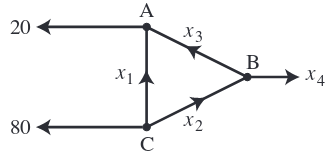
\includegraphics[width=2in]{figures/1_6_11.png}
        \end{center}
    \end{figure}

    \begin{solution}
        The inputs and outputs of each node in the network can be described as
        \begin{align*}
            A: x_3 + x_2 = 20 \\
            B: x_2 = x_3 + x_4 \\
            C: 80 = x_1 + x_2
        \end{align*}

        This is equivalent to the following agumented matrices
        \begin{align*}
            \begin{Mat}
                1 & 0 & 1 & 0 & 20 \\
                0 & -1 & 1 & 1 & 0 \\
                1 & 1 & 0 & 0 & 80
            \end{Mat} & \equiv
            \begin{Mat}
                1 & 0 & 1 & 0 & 20 \\
                0 & -1 & 1 & 1 & 0 \\
                0 & 1 & -1 & 0 & 60
            \end{Mat} & R_3 = R_3 - R_1 \\ & \equiv
            \begin{Mat}
                1 & 0 & 1 & 0 & 20 \\
                0 & -1 & 1 & 1 & 0 \\
                0 & 0 & 0 & 1 & 60
            \end{Mat} & R_3 = R_3 + R_2 \\ & \equiv
            \begin{Mat}
                1 & 0 & 1 & 0 & 20 \\
                0 & -1 & 1 & 0 & -60 \\
                0 & 0 & 0 & 1 & 60
            \end{Mat} & R_2 = R_2 - R_3 \\ & \equiv
            \begin{Mat}
                1 & 0 & 1 & 0 & 20 \\
                0 & 1 & -1 & 0 & 60 \\
                0 & 0 & 0 & 1 & 60
            \end{Mat} & R_2 = -R_2
        \end{align*}

        So the network can be described by the system
        \begin{align*}
            x_1 &= 20 - x_3 \\
            x_2 &= 60 + x_3 \\
            x_3 &= x_3 \\
            x_4 &= 60
        \end{align*}

        The largest possible value of $x_3$ for all nonnegative flows is $20$.
    \end{solution}
\end{problem}

\newpage

\begin{problem}[1.6\#13]
    \begin{enumerate}[label=\alph*.]
        \item Find the general flow pattern in the network shown in the figure.
        \item Assuming that the flow must be in the directions indicated, find the minimum flows in the branches denoted by $x_2,x_3,x_4$ and $x_5$.
    \end{enumerate}

    \begin{figure}[h!]
        \begin{center}
            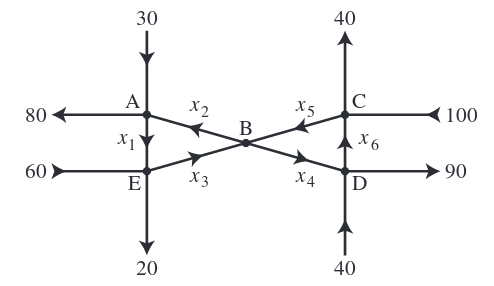
\includegraphics[width=3in]{figures/1_6_13.png}
        \end{center}
    \end{figure}


    \begin{solution}[Part A:]
        The inputs and outputs of each node in the network can be described as
        \begin{align*}
            A:& 30 + x_2 = 80 + x_1 \\
            B:& x_3 + x_5 = x_2 + x_4 \\
            C:& 100 + x_6 = x_5 + 40 \\
            D:& x_4 + 40 = x_6 + 90 \\
            E:& x_1 + 60 = 20 + x_3
        \end{align*}

        This is equivalent to the following augmented matrices
        \begin{align*}
            \begin{Mat}
                -1 & 1 & 0 & 0 & 0 & 0 & 50 \\ 
                0 & -1 & 1 & -1 & 1 & 0 & 0 \\
                0 & 0 & 0 & 0 & -1 & 1 & -60 \\
                0 & 0 & 0 & 1 & 0 & -1 & 50 \\ 
                1 & 0 & -1 & 0 & 0 & 0 & -40
            \end{Mat}
            & \equiv \begin{Mat}
                -1 & 1 & 0 & 0 & 0 & 0 & 50 \\ 
                0 & -1 & 1 & -1 & 1 & 0 & 0 \\
                0 & 0 & 0 & 0 & -1 & 1 & -60 \\
                0 & 0 & 0 & 1 & 0 & -1 & 50 \\ 
                0 & 1 & -1 & 0 & 0 & 0 & 10
            \end{Mat} 
            \\
            & \qquad{} R5 = R5 + R_1 \\
            \equiv \begin{Mat}
                -1 & 1 & 0 & 0 & 0 & 0 & 50 \\ 
                0 & -1 & 1 & -1 & 1 & 0 & 0 \\
                0 & 0 & 0 & 0 & -1 & 1 & -60 \\
                0 & 0 & 0 & 1 & 0 & -1 & 50 \\ 
                0 & 0 & 0 & -1 & 1 & 0 & 10
            \end{Mat}
            & \equiv \begin{Mat}
                -1 & 1 & 0 & 0 & 0 & 0 & 50 \\ 
                0 & -1 & 1 & -1 & 1 & 0 & 0 \\
                0 & 0 & 0 & 0 & -1 & 1 & -60 \\
                0 & 0 & 0 & 1 & 0 & -1 & 50 \\ 
                0 & 0 & 0 & 0 & 1 & -1 & 60
            \end{Mat}
            \\ 
            R5 = R5 + R_2 & \qquad{} R5 = R5 + R_4 \\ 
            \equiv \begin{Mat}
                -1 & 1 & 0 & 0 & 0 & 0 & 50 \\ 
                0 & -1 & 1 & -1 & 1 & 0 & 0 \\
                0 & 0 & 0 & 0 & -1 & 1 & -60 \\
                0 & 0 & 0 & 1 & 0 & -1 & 50 \\ 
                0 & 0 & 0 & 0 & 0 & 0 & 0
            \end{Mat}
            & \equiv 
            \begin{Mat}
                -1 & 1 & 0 & 0 & 0 & 0 & 50 \\ 
                0 & -1 & 1 & -1 & 1 & 0 & 0 \\
                0 & 0 & 0 & 1 & 0 & -1 & 50 \\ 
                0 & 0 & 0 & 0 & -1 & 1 & -60 \\
                0 & 0 & 0 & 0 & 0 & 0 & 0
            \end{Mat}
            \\ 
            R5 = R5 + R_3 & \qquad{} \text{Swap $R_3$ \& $R_4$} \\
            \equiv \begin{Mat}
                -1 & 1 & 0 & 0 & 0 & 0 & 50 \\ 
                0 & -1 & 1 & -1 & 1 & 0 & 0 \\
                0 & 0 & 0 & 1 & 0 & -1 & 50 \\ 
                0 & 0 & 0 & 0 & 1 & -1 & 60 \\
                0 & 0 & 0 & 0 & 0 & 0 & 0
            \end{Mat}
            & \equiv \begin{Mat}
                1 & -1 & 0 & 0 & 0 & 0 & -50 \\ 
                0 & -1 & 1 & -1 & 1 & 0 & 0 \\
                0 & 0 & 0 & 1 & 0 & -1 & 50 \\ 
                0 & 0 & 0 & 0 & 1 & -1 & 60 \\
                0 & 0 & 0 & 0 & 0 & 0 & 0
            \end{Mat}
            \\ 
            R_4 = -R_4 & \qquad{} R_1 = -R_1 \\
            \equiv \begin{Mat}
                1 & -1 & 0 & 0 & 0 & 0 & -50 \\ 
                0 & 1 & -1 & 1 & -1 & 0 & 0 \\
                0 & 0 & 0 & 1 & 0 & -1 & 50 \\ 
                0 & 0 & 0 & 0 & 1 & -1 & 60 \\
                0 & 0 & 0 & 0 & 0 & 0 & 0
            \end{Mat}
            & \equiv \begin{Mat}
                1 & -1 & 0 & 0 & 0 & 0 & -50 \\ 
                0 & 1 & -1 & 1 & 0 & -1 & 60 \\
                0 & 0 & 0 & 1 & 0 & -1 & 50 \\ 
                0 & 0 & 0 & 0 & 1 & -1 & 60 \\
                0 & 0 & 0 & 0 & 0 & 0 & 0
            \end{Mat}
            \\ 
            R_2 = -R_2 & \qquad{} R_2 = R_2 + R_4 \\ 
            \equiv \begin{Mat}
                1 & -1 & 0 & 0 & 0 & 0 & -50 \\ 
                0 & 1 & -1 & 0 & 0 & 0 & 10 \\
                0 & 0 & 0 & 1 & 0 & -1 & 50 \\ 
                0 & 0 & 0 & 0 & 1 & -1 & 60 \\
                0 & 0 & 0 & 0 & 0 & 0 & 0
            \end{Mat}
            & \equiv 
            \begin{Mat}
                1 & 0 & -1 & 0 & 0 & 0 & -40 \\ 
                0 & 1 & -1 & 0 & 0 & 0 & 10 \\
                0 & 0 & 0 & 1 & 0 & -1 & 50 \\ 
                0 & 0 & 0 & 0 & 1 & -1 & 60 \\
                0 & 0 & 0 & 0 & 0 & 0 & 0
            \end{Mat}
            \\ 
            R_2 = R_2 - R_3 & \qquad{} R_1 = R_1 + R_2
        \end{align*}

        So the network can be described by the system
        \begin{align*}
            x_1 = x_3 - 40 \\ 
            x_2 = x_3 + 10 \\ 
            x_3 = x_3 \\ 
            x_4 = x_6 + 50 \\ 
            x_5 = x_6 + 60 \\ 
            x_6 = x_6
        \end{align*}
    \end{solution}

    \begin{solution}[Part B:]
        The minimum flows for $x_2, x_3, x_4$ and $x_5$ are $x_2 = 50, x_3 = 40, x_4 = 50, x_5 = 60$.
    \end{solution}
\end{problem}

\begin{problem}[1.7\#1]
    Determine if the vectors are linearly independent. Justify answer.
    
    \begin{equation*}
        \begin{Mat}
            5 \\ 0 \\ 0
        \end{Mat},
        \begin{Mat}
            7 \\ 2 \\ -6
        \end{Mat},
        \begin{Mat}
            9 \\ 4 \\ -8
        \end{Mat}
    \end{equation*}

    \begin{solution}
        \begin{align*}
            \begin{Mat}
                5 & 7 & 9 \\
                0 & 2 & 4 \\
                0 & -6 & -8
            \end{Mat} 
            & \equiv \begin{Mat}
                5 & 7 & 9 \\
                0 & 2 & 4 \\
                0 & 0 & 4
            \end{Mat} 
            \\ 
            & \qquad{} R_3 = R_3 + 3R_2 \\
            \equiv \begin{Mat}
                5 & 7 & 9 \\
                0 & 1 & 2 \\
                0 & 0 & 4
            \end{Mat}
            & \equiv \begin{Mat}
                5 & 7 & 9 \\
                0 & 1 & 2 \\
                0 & 0 & 1
            \end{Mat}
            \\ 
            R_2 = R_2/2 & \qquad{} R_3 = R_3/4 \\
            \equiv \begin{Mat}
                5 & 7 & 9 \\
                0 & 1 & 0 \\
                0 & 0 & 1
            \end{Mat}
            & \equiv \begin{Mat}
                5 & 7 & 0 \\
                0 & 1 & 0 \\
                0 & 0 & 1
            \end{Mat}
            \\
            R_2 = R_2 - R_3 & \qquad{} R_1 = R_1 - 9R_3 \\ 
            \equiv \begin{Mat}
                5 & 0 & 0 \\
                0 & 1 & 0 \\
                0 & 0 & 1
            \end{Mat}
            & \equiv \begin{Mat}
                1 & 0 & 0 \\
                0 & 1 & 0 \\
                0 & 0 & 1
            \end{Mat}
            \\ 
            R_1 = R_1 - 7R_2 & \qquad{} R_1 = R_1/5
        \end{align*}

        The vectors are linearly independent, because their coefficent matrix has a pivot point in each row.
    \end{solution}
\end{problem}

\newpage

\begin{problem}[1.7\#3]
    Determine if the vectors are linearly independent. Justify answer.
    
    \begin{equation*}
        \begin{Mat}
            1 \\ -3
        \end{Mat},
        \begin{Mat}
            -3 \\ 9
        \end{Mat}
    \end{equation*}

    \begin{solution}
        The vectors are linearly dependent because $\begin{Mat}-3 \\ 9\end{Mat} = -3\begin{Mat}1 \\ -3\end{Mat}$.
    \end{solution}
\end{problem}

\begin{problem}[1.7\#5]
    Determine if the columns of the matrix form a linearly independent set. Justify your answer.

    \begin{equation*}
        \begin{Mat}
            0 & -8 & 5 \\
            3 & -7 & 4 \\
            -1 & 5 & -4 \\
            1 & -3 & 2
        \end{Mat}
    \end{equation*}

    \begin{solution}
        \begin{align*}
            \begin{Mat}
                0 & -8 & 5 \\
                3 & -7 & 4 \\
                -1 & 5 & -4 \\
                1 & -3 & 2
            \end{Mat}
            & \equiv \begin{Mat}
                1 & -3 & 2 \\ 
                3 & -7 & 4 \\
                -1 & 5 & -4 \\
                0 & -8 & 5
            \end{Mat}
            \\ 
            & \qquad{} \text{Swap $R_1$ \& $R_4$} \\
            \equiv \begin{Mat}
                1 & -3 & 2 \\ 
                3 & -7 & 4 \\
                0 & 2 & -2 \\
                0 & -8 & 5
            \end{Mat}
            & \equiv \begin{Mat}
                1 & -3 & 2 \\ 
                0 & 2 & -2 \\
                0 & 2 & -2 \\
                0 & -8 & 5
            \end{Mat}
            \\ 
            R_3 = R_3 + R_1 & \qquad{} R_2 = R_2 - 3R_1 \\
            \equiv \begin{Mat}
                1 & -3 & 2 \\ 
                0 & 2 & -2 \\
                0 & 0 & 0 \\
                0 & -8 & 5
            \end{Mat} 
            & \equiv \begin{Mat}
                1 & -3 & 2 \\ 
                0 & 2 & -2 \\
                0 & -8 & 5 \\
                0 & 0 & 0 \\
            \end{Mat} 
            \\ 
            R_3 = R_3 - R_2 & \qquad{} \text{Swap $R_3$ \& $R_4$} \\
            \equiv \begin{Mat}
                1 & -3 & 2 \\ 
                0 & 2 & -2 \\
                0 & 0 & -3 \\
                0 & 0 & 0 \\
            \end{Mat}
            & \equiv \begin{Mat}
                1 & -3 & 2 \\ 
                0 & 2 & -2 \\
                0 & 0 & 1 \\
                0 & 0 & 0 \\
            \end{Mat}
            \\ 
            R_3 = R_3 + 4R_2 & \qquad{} R_3 = -R_3/3
        \end{align*}

        The columns do form a linearly independent set because there is only the trivial solution to $A\Vect{x} = 0$.
    \end{solution}
\end{problem}

\begin{problem}[1.7\#7]
    Determine if the columns of the matrix form a linearly independent set. Justify your answer.

    \begin{equation*}
        \begin{Mat}
            1 & 4 & -3 & 0 \\
            -2 & -7 & 5 & 1 \\
            -4 & -5 & 7 & 5
        \end{Mat}
    \end{equation*}

    \begin{solution}
        The columns do not form a linearly independent set because the coefficent matrix is underdetermined, and will therefore have a free variable.
    \end{solution}
\end{problem}

\begin{problem}[1.7\#11]
    Find the value(s) of $h$ for which the vectors are linearly dependent. Justify your answer.

    \begin{equation*}
        \begin{Mat}
            1 \\ -1 \\ 4
        \end{Mat},
        \begin{Mat}
            3 \\ -5 \\ 7
        \end{Mat},
        \begin{Mat}
            -1 \\ 5 \\ h
        \end{Mat}
    \end{equation*}

    \begin{solution}
        \begin{align*}
            \begin{Mat}
                1 & 3 & -1 \\ 
                -1 & -5 & 5 \\ 
                4 & 7 & h
            \end{Mat} & \equiv
            \begin{Mat}
                1 & 3 & -1 \\ 
                0 & -2 & 4 \\ 
                4 & 7 & h
            \end{Mat} & R_2 = R_2 + R_1 \\ & \equiv
            \begin{Mat}
                1 & 3 & -1 \\ 
                0 & -2 & 4 \\ 
                0 & -5 & h + 4
            \end{Mat} & R_3 = R_3 - 4R_1 \\ & \equiv
            \begin{Mat}
                1 & 3 & -1 \\ 
                0 & 1 & -2 \\ 
                0 & -5 & h + 4
            \end{Mat} & R_2 = -\frac{R_2}{2} \\ & \equiv
            \begin{Mat}
                1 & 3 & -1 \\ 
                0 & 1 & -2 \\ 
                0 & 0 & h - 6
            \end{Mat} & R_3 = R_3 + 5R_2
        \end{align*}

        The vectors will be linearly dependent if $h = 6$, because if $h = 6$ then there is a free variable.
    \end{solution}
\end{problem}

\newpage

\begin{problem}[1.7\#13]
    Find the value(s) of $h$ for which the vectors are linearly dependent. Justify your answer.

    \begin{equation*}
        \begin{Mat}
            1 \\ 5 \\ -3
        \end{Mat},
        \begin{Mat}
            -2 \\ -9 \\ 6
        \end{Mat},
        \begin{Mat}
            3 \\ h \\ -9
        \end{Mat}
    \end{equation*}

    \begin{solution}
        \begin{align*}
            \begin{Mat}
                1 & -2 & 3 \\ 
                5 & -9 & h \\ 
                -3 & 6 & -9
            \end{Mat} & \equiv
            \begin{Mat}
                1 & -2 & 3 \\ 
                5 & -9 & h \\ 
                0 & 0 & 0
            \end{Mat} & R_3 = R_3 + 3R_1
        \end{align*}

        The vectors will be linearly dependent for all possible value of $h$, because there is already a free varaible regardless of the value of $h$.
    \end{solution}
\end{problem}

\begin{problem}[1.7\#15]
    Determine by inspection whether the vectors are linearly independent. Justify your answer.

    \begin{equation*}
        \begin{Mat}
            5 \\ 1
        \end{Mat},
        \begin{Mat}
            2 \\ 8
        \end{Mat},
        \begin{Mat}
            1 \\ 3
        \end{Mat},
        \begin{Mat}
            -1 \\ 7
        \end{Mat}
    \end{equation*}

    \begin{solution}
        The vectors are linearly independent, because no vector is equal to the scalar multiple of another.
    \end{solution}
\end{problem}

\newpage

\begin{problem}[1.7\#17]
    Determine by inspection whether the vectors are linearly independent. Justify your answer.

    \begin{equation*}
        \begin{Mat}
            3 \\ 5 \\ -1
        \end{Mat},
        \begin{Mat}
            0 \\ 0 \\ 0
        \end{Mat},
        \begin{Mat}
            -6 \\ 5 \\ 4
        \end{Mat}
    \end{equation*}

    \begin{solution}
        \begin{align*}
            \begin{Mat}
                3 & 0 & -6 \\ 
                5 & 0 & 5 \\ 
                -1 & 0 & 4 \\
            \end{Mat}
            & \equiv \begin{Mat}
                1 & 0 & -2 \\ 
                5 & 0 & 5 \\ 
                -1 & 0 & 4 \\
            \end{Mat}
            \\ 
            & \qquad{} R_1 = R_1/3 \\ 
            \equiv \begin{Mat}
                1 & 0 & -2 \\ 
                1 & 0 & 1 \\ 
                -1 & 0 & 4 \\
            \end{Mat}
            & \equiv \begin{Mat}
                1 & 0 & -2 \\ 
                1 & 0 & 1 \\ 
                0 & 0 & 2 \\
            \end{Mat}
            \\ 
            R_2 = R_2/5 & \qquad{} R_3 = R_3 + R_1 \\
            \equiv \begin{Mat}
                1 & 0 & -2 \\ 
                0 & 0 & 3 \\ 
                0 & 0 & 2 \\
            \end{Mat}
            & \equiv \begin{Mat}
                1 & 0 & -2 \\ 
                0 & 0 & 3 \\ 
                0 & 0 & 0 \\
            \end{Mat}
            \\
            R_2 = R_2 - R_1 & \qquad{} R_3 = R_3 - 2R_2/3
        \end{align*}

        The vectors are linearly dependent because there is not a pivot point in each row of the coefficent matrix formed by the vectors.
    \end{solution}
\end{problem}

\begin{problem}[1.7\#19]
    Determine by inspection whether the vectors are linearly independent. Justify your answer.

    \begin{equation*}
        \begin{Mat}
            -8 \\ 12 \\ -4
        \end{Mat},
        \begin{Mat}
            2 \\ -3 \\ -1
        \end{Mat}
    \end{equation*}

    \begin{solution}
        Yes, the vectors are linearly independent because they are not multiples of each other.
    \end{solution}
\end{problem}

\begin{problem}[1.7\#21]
    Mark each statment True or False. Justify each answer on the basis of a careful reading of the text.
    
    \begin{enumerate}[label=(\alph*)]
        \item The columns of a matrix $A$ are linearly independent if the equation $A\Vect{x} = 0$ has the trivial solution
        \item If $S$ is a linearly dependent set, then each vector is a linear combination of the other vectors in $S$.
        \item The columns of any $4 \times 5$ matrix are linearly dependent.
        \item If $x$ and $y$ are linearly independent, and if $\{x,y,z\}$ is linearly dependent, then $z$ is in $\Span{x,y}$
    \end{enumerate}

    \begin{solution}
        \begin{enumerate}[label=(\alph*)]
            \item \underline{False}, the columns maybe linearly independent, but having the trivial solution does not imply that they are linearly independent.
            \item \underline{False}, for the vectors in $S$ to be linearly independent, they cannot be linear combinations of the other vectors in the set.
            \item \underline{True}, a $4 \times 5$ matrix is underdetermined, and therefore it's columns are a linearly dependent.
            \item \underline{True}, if $\{x,y,z\}$ is linearly dependent, then $z$ can be written as a linear combination of $x$ and $y$, and therefore is in $\Span{x,y}$.
        \end{enumerate}
    \end{solution}
\end{problem}

\begin{problem}[1.7\#23]
    Describe the possible echelon forms of $A$, a $3 \times 3$ matrix with linearly independent columns. Use the notation of Example 1 in Section 1.2

    \begin{solution}
        \begin{align*}
            \begin{Mat}
                \blacksquare & * & * \\ 
                0 & \blacksquare & * \\
                0 & 0 & \blacksquare
            \end{Mat}
        \end{align*}
    \end{solution}
\end{problem}

\begin{problem}[1.7\#25]
    Describe the possible echelon forms of $A = [\Vect{a_1}, \Vect{a_2}]$, a $4 \times 2$ matrix, such that $\Vect{a_2}$ is not a multiple of $\Vect{a_1}$ with linearly dependent columns. Use the notation of Example 1 in Section 1.2

    \begin{solution}
        \begin{equation*}
            \begin{Mat}
                \blacksquare & * \\ 
                0 & \blacksquare \\ 
                0 & 0 \\ 
                0 & 0
            \end{Mat}
        \end{equation*}
    \end{solution}
\end{problem}

\begin{problem}[1.8\#1]
    Let $A = \begin{Mat}
        2 & 0 \\
        0 & 2
    \end{Mat}$, and define $T: \R^2 \to R^2$ by $T(\Vect{x}) = A\Vect{x}$. Find the images under $T$ of $\Vect{u} = \begin{Mat}
        1 \\ -3
    \end{Mat}$, and $\Vect{v} = \begin{Mat}
        a \\ b
    \end{Mat}$.

    \begin{solution}
        \begin{equation*}
            T(\Vect{u}) = \begin{Mat}
                2 & 0 \\ 
                0 & 2
            \end{Mat} \begin{Mat}
                1 \\ -3
            \end{Mat} = \begin{Mat}
                2 \\ -6
            \end{Mat}
        \end{equation*}

        \begin{equation*}
            T(\Vect{v}) = \begin{Mat}
                2 & 0 \\ 
                0 & 2
            \end{Mat} \begin{Mat}
                a \\ b
            \end{Mat} = \begin{Mat}
                2a \\ 2b
            \end{Mat}
        \end{equation*}
    \end{solution}
\end{problem}

\begin{problem}[1.8\#2]
    Let $A = \begin{Mat}
        .5 & 0 & 0 \\
        0 & .5 & 0 \\
        0 & 0 & .5 \\
    \end{Mat}, \Vect{u} = \begin{Mat}
        1 \\ 0 \\ -4
    \end{Mat}$, and $\Vect{v} = \begin{Mat}
        a \\ b \\ c
    \end{Mat}$. Define $T: \R^3 \to R^3$ by $T(\Vect{x}) = A\Vect{x}$. Find $T(\Vect{u})$ and $T(\Vect{v})$.

    \begin{solution}
        \begin{equation*}
            T(\Vect{u}) = \begin{Mat}
                .5 & 0 & 0 \\
                0 & .5 & 0 \\
                0 & 0 & .5 \\
            \end{Mat} \begin{Mat}
                1 \\ 0 \\ -4
            \end{Mat} = \begin{Mat}
                0.5 \\ 0 \\ -2
            \end{Mat}
        \end{equation*}

        \begin{equation*}
            T(\Vect{v}) = \begin{Mat}
                .5 & 0 & 0 \\
                0 & .5 & 0 \\
                0 & 0 & .5 \\
            \end{Mat} \begin{Mat}
                a \\ b \\ c
            \end{Mat} = \begin{Mat}
                0.5a \\ 0.5b \\ 0.5c
            \end{Mat}
        \end{equation*}
    \end{solution}
\end{problem}

\begin{problem}[1.8\#3]
    Find a vector $\Vect{x}$ whose image under $T$ is $\Vect{b}$ and determine whether $x$ is unique. $T(\Vect{x}) = A\Vect{x}$.
    \begin{equation*}
        A = \begin{Mat}
            1 & 0 & -2 \\
            -2 & 1 & 6 \\
            3 & -2 & -5
        \end{Mat},
        \Vect{b} = \begin{Mat}
            -1 \\ 7 \\ -3
        \end{Mat}
    \end{equation*}

    \begin{solution}
        \begin{align*}
            \begin{Mat}
                1 & 0 & -2 & -1\\
                -2 & 1 & 6 & 7\\
                3 & -2 & -5 & -3
            \end{Mat} 
            & \equiv \begin{Mat}
                1 & 0 & -2 & -1\\
                0 & 1 & 2 & 5\\
                3 & -2 & -5 & -3
            \end{Mat}
            \\ 
            & \qquad{} R_2 = R_2 + 2R_1 \\
            \equiv \begin{Mat}
                1 & 0 & -2 & -1\\
                0 & 1 & 2 & 5\\
                0 & -2 & 1 & 0
            \end{Mat}
            & \equiv \begin{Mat}
                1 & 0 & -2 & -1\\
                0 & 1 & 2 & 5\\
                0 & 0 & 5 & 10
            \end{Mat}
            \\ 
            R_3 = R_3 - 3R_1 & \qquad{} R_3 = R_3 + 2R_2 \\
            \equiv \begin{Mat}
                1 & 0 & -2 & -1\\
                0 & 1 & 2 & 5\\
                0 & 0 & 1 & 2
            \end{Mat}
            & \equiv \begin{Mat}
                1 & 0 & -2 & -1\\
                0 & 1 & 0 & 1\\
                0 & 0 & 1 & 2
            \end{Mat}
            \\ 
            R_3 = R_3/5 & \qquad{} R_2 = R_2 - R_3 \\
            \equiv \begin{Mat}
                1 & 0 & 0 & 3\\
                0 & 1 & 0 & 1\\
                0 & 0 & 1 & 2
            \end{Mat} 
            \\
            R_1 = R_1 + 2R_3
        \end{align*}

        The vector $\Vect{x}$ whose image under $T$ is $\Vect{b}$ is unique and is equal to $\begin{Mat}
            3 \\ 1 \\ 2
        \end{Mat}$.
    \end{solution}
\end{problem}

\begin{problem}[1.8\#5]
    Find a vector $\Vect{x}$ whose image under $T$ is $\Vect{b}$ and determine whether $x$ is unique. $T(\Vect{x}) = A\Vect{x}$.
    \begin{equation*}
        A = \begin{Mat}
            1 & -5 & -7 \\
            -3 & 7 & 5
        \end{Mat},
        \Vect{b} = \begin{Mat}
            -2 \\ -2
        \end{Mat}
    \end{equation*}

    \begin{solution}
        \begin{align*}
            \begin{Mat}
                1 & -5 & -7 & -2\\
                -3 & 7 & 5 & -2
            \end{Mat} & \equiv
            \begin{Mat}
                1 & -5 & -7 & -2\\
                0 & -8 & -16 & -8
            \end{Mat} & R_2 = R_2 + 3R_1 \\ & \equiv
            \begin{Mat}
                1 & -5 & -7 & -2\\
                0 & 1 & 2 & 1
            \end{Mat} & R_2 = -\frac{R_2}{8} \\ & \equiv
            \begin{Mat}
                1 & 0 & 3 & 3\\
                0 & 1 & 2 & 1
            \end{Mat} & R_1 = R_1 + 5R_2 \\ & \equiv
            \begin{Bmatrix}
                x_1 = 3 - 3x_3 \\ 
                x_2 = 1 - 2x_3
            \end{Bmatrix}
        \end{align*}

        The vectors whose image under $T$ is $\Vect{b}$ are
        \begin{equation*}
            \Vect{x} = x_3\begin{Mat}
                -3 \\ -2 \\ 1
            \end{Mat} + \begin{Mat}
                3 \\ 1 \\ 0
            \end{Mat}
        \end{equation*}

        One such vector is $\begin{Mat}
            3 \\ 1 \\ 0
        \end{Mat}$, but it is not a unique solution.
    \end{solution}
\end{problem}

\begin{problem}[1.8\#7]
    Let $A$ be $6 \times 5$ matrix. What must $a$ and $b$ be in order to define $T: \R^a \to \R^b$ by $T(x) = A\Vect{x}$?

    \begin{solution}
        \begin{equation*}
            a = 5, b = 6
        \end{equation*}
    \end{solution}
\end{problem}

\newpage

\begin{problem}[1.8\#9]
    Find all $x$ in $\R^4$ that are mapped into the zero vector by the transofmration $\Vect{x} \mapsto A\Vect{x}$ for the given matrix $A$.
    
    \begin{equation*}
        \begin{Mat}
            1 & -4 & 7 & -5 \\
            0 & 1 & -4 & 3 \\
            2 & -6 & 6 & -4
        \end{Mat}
    \end{equation*}

    \begin{solution}
        \begin{align*}
            \begin{Mat}
                1 & -4 & 7 & -5 & 0 \\
                0 & 1 & -4 & 3 & 0 \\
                2 & -6 & 6 & -4 & 0
            \end{Mat}
            & \equiv \begin{Mat}
                1 & -4 & 7 & -5 & 0 \\
                0 & 1 & -4 & 3 & 0 \\
                0 & 2 & -8 & 6 & 0
            \end{Mat}
            \\ 
            & \qquad{} R_3 = R_3 - 2R_1 \\
            \equiv \begin{Mat}
                1 & -4 & 7 & -5 & 0 \\
                0 & 1 & -4 & 3 & 0 \\
                0 & 0 & 0 & 0 & 0
            \end{Mat}
            & \equiv \begin{Mat}
                1 & 0 & -9 & 7 & 0 \\
                0 & 1 & -4 & 3 & 0 \\
                0 & 0 & 0 & 0 & 0
            \end{Mat}
            \\ R_3 = R_3 - 2R_2 & \qquad{} R_1 = R_1 + 4R_2 \\
            \equiv \begin{Bmatrix}
                x_1 = 9x_3 - 7x_4 \\ 
                x_2 = 4x_3 - 3x_4 \\ 
                x_3 = x_3 \\ 
                x_4 = x_4
            \end{Bmatrix}
        \end{align*}

        The \Vect{x} in $\R^4$ that are mapped into the zero vector by $A$ are...
        \begin{equation*}
            \Vect{x} = x_3\begin{Mat}
                9 \\ 4 \\ 1 \\ 0
            \end{Mat} + x_4\begin{Mat}
                -7 \\ -3 \\ 0 \\ 1
            \end{Mat}
        \end{equation*}
    \end{solution}
\end{problem}

\newpage

\begin{problem}[1.8\#11]
    Let $\Vect{b} = \begin{Mat}
        -1 \\ 1 \\ 0
    \end{Mat}$, and let $A$ be the matrix be the matrix in Exercise 9. Is $\Vect{b}$ in the range of the linear transofmration $\Vect{x} \mapsto A\Vect{x}$? Why or why not?

    \begin{solution}
        \begin{align*}
            \begin{Mat}
                1 & -4 & 7 & -5 & -1 \\
                0 & 1 & -4 & 3 & 1 \\
                2 & -6 & 6 & -4 & 0
            \end{Mat} 
            & \equiv \begin{Mat}
                1 & -4 & 7 & -5 & -1 \\
                0 & 1 & -4 & 3 & 1 \\
                0 & 2 & -8 & 6 & 2
            \end{Mat} 
            \\ 
            & \qquad{} R_3 = R_3 - 2R_1 \\
            \equiv \begin{Mat}
                1 & -4 & 7 & -5 & -1 \\
                0 & 1 & -4 & 3 & 1 \\
                0 & 0 & 0 & 0 & 0
            \end{Mat}
            & \equiv \begin{Mat}
                1 & 0 & -9 & 7 & 3 \\
                0 & 1 & -4 & 3 & 1 \\
                0 & 0 & 0 & 0 & 0
            \end{Mat}
            \\ 
            R_3 = R_3 - 2R_2 & \qquad{} R_1 = R_1 + 4R_2 \\
            \equiv \begin{Bmatrix}
                x_1 = 9x_3 - 7x_4 + 3 \\ 
                x_2 = 4x_3 - 3x_4 + 1 \\ 
                x_3 = x_3 \\ 
                x_4 = x_4
            \end{Bmatrix}
        \end{align*}

        Yes, $\Vect{b}$ is in the range of the linear transformation $\Vect{x} \mapsto A\Vect{x}$ because the system $A\Vect{x} = \Vect{b}$ is consistent.
    \end{solution}
\end{problem}

\newpage

\begin{problem}[1.8\#13]
    Use a rectangular coordinate system to plot $\Vect{u} = \begin{Mat}
        5 \\ 2
    \end{Mat}$, $\Vect{v} = \begin{Mat}
        -2 \\ 4
    \end{Mat}$, and their images under the given transformation $T$. Describe geometrically what $T$ does to each vector $x$ in $\R^2$.

    \begin{equation*}
        T(\Vect{x}) = \begin{Mat}
            -1 & 0 \\
            0 & -1
        \end{Mat}
        \begin{Mat}
            x_1 \\ x_2
        \end{Mat}
    \end{equation*}

    \begin{solution}
        \begin{figure}[h!]
            \begin{center}
                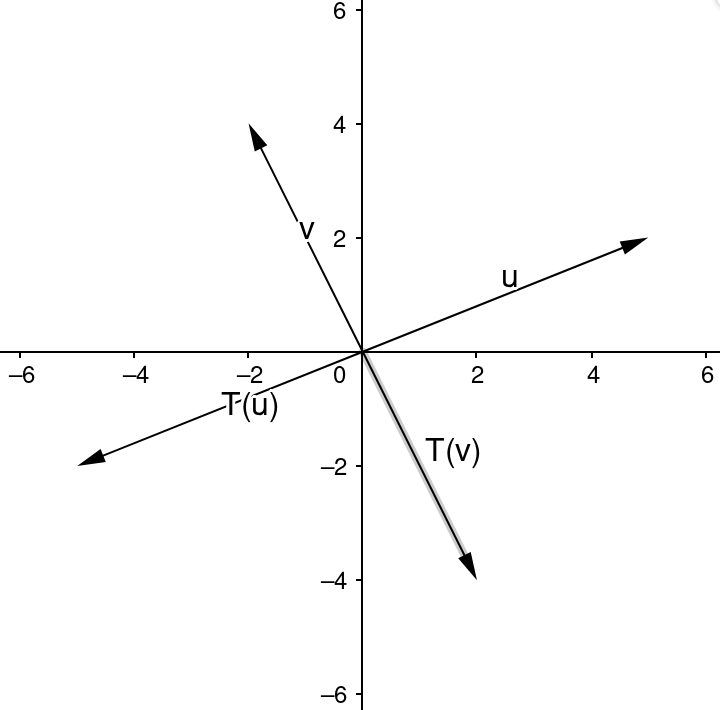
\includegraphics[width=3in]{figures/1_8_13_solution.png}
            \end{center}
        \end{figure}
        
        $T$ reflects each vector across the origin
    \end{solution}
\end{problem}

\newpage

\begin{problem}[1.8\#16]
    Use a rectangular coordinate system to plot $\Vect{u} = \begin{Mat}
        5 \\ 2
    \end{Mat}$, $\Vect{v} = \begin{Mat}
        -2 \\ 4
    \end{Mat}$, and their images under the given transformation $T$. Describe geometrically what $T$ does to each vector $x$ in $\R^2$.

    \begin{equation*}
        T(\Vect{x}) = \begin{Mat}
            0 & 1 \\
            1 & 0
        \end{Mat}
        \begin{Mat}
            x_1 \\ x_2
        \end{Mat}
    \end{equation*}

    \begin{solution}
        \begin{figure}[h!]
            \begin{center}
                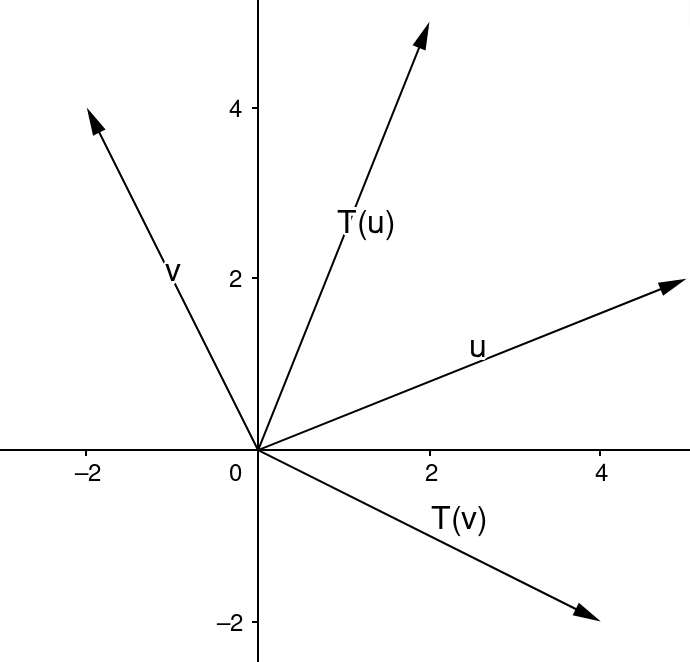
\includegraphics[width=3in]{figures/1_8_16_solution.png}
            \end{center}
        \end{figure}
    \end{solution}

    $T$ swaps the $x_1$ and $x_2$ components of each vector.
\end{problem}

\begin{problem}[1.8\#30]
    An \textit{affine transofmration} $T: \R^n \to R^m$ has the form $T(\Vect{x}) = A\Vect{x} + \Vect{b}$, with $A$ an $m \times n$ matrix and $\Vect{b}$ in $\R^m$.
    Show that $T$ is \textit{not} a linear transofmation when $\Vect{b} \neq 0$ 

    \begin{solution}
        \begin{proof}
            Show that $T(c\Vect{x}) \neq cT(\Vect{x})$
            \begin{align}
                T(c\Vect{x}) & = A(c\Vect{x}) + \Vect{b} \\
                cT(\Vect{x}) & = c(A\Vect{x} + \Vect{b}) \\
                    & = A(c\Vect{x}) + c\Vect{b} \\
                A(c\Vect{x}) + \Vect{b} &\neq A(c\Vect{x}) + c\Vect{b}
            \end{align}

            Because it does not hold true that $T(c\Vect{x}) = cT(\Vect{x})$ for the transformation $T(\Vect{x}) = A\Vect{x} + \Vect{b}$ it is not a linear transformation.
        \end{proof}
    \end{solution}
\end{problem}

\begin{problem}[1.8\#33]
    Show that the transformation $T$ defined by $T(x_1,x_2) = (2x_1 - 3x_2, x_1 + 4, 5x_2)$ is not linear.

    \begin{solution}
        \begin{proof}
            Show that $T(c\Vect{x}) \neq cT(\Vect{x})$
            \begin{align}
                T(cx_1,cx_2) & = (2cx_1 - 3cx_2, cx_1 + 4, 5cx_2)\\
                cT(\Vect{x}) & = c(2x_1 - 3x_2, x_1 + 4, 5x_2) \\
                    & = (2cx_1 - 3cx_2, cx_1 + c4, 5cx_2) \\
                (2cx_1 - 3cx_2, cx_1 + 4, 5cx_2) &\neq (2cx_1 - 3cx_2, cx_1 + c4, 5cx_2) 
            \end{align}

            Because it does not hold true that $T(c\Vect{x}) = cT(\Vect{x})$ for the transformation $T(\Vect{x}) = (2x_1 - 3x_2, x_1 + 4, 5x_2)$ it is not a linear transformation.
        \end{proof}
    \end{solution}
\end{problem}

\end{document}